		
%% abtex2-modelo-trabalho-academico.tex, v-1.9.3 laurocesar
%% Copyright 2012-2015 by abnTeX2 group at http://abntex2.googlecode.com/ 
%%
%% This work may be distributed and/or modified under the
%% conditions of the LaTeX Project Public License, either version 1.3
%% of this license or (at your option) any later version.
%% The latest version of this license is in
%%   http://www.latex-project.org/lppl.txt
%% and version 1.3 or later is part of all distributions of LaTeX
%% version 2005/12/01 or later.
%%
%% This work has the LPPL maintenance status `maintained'.
%% 
%% The Current Maintainer of this work is the abnTeX2 team, led
%% by Lauro César Araujo. Further information are available on 
%% http://abntex2.googlecode.com/
%%
%% This work consists of the files abntex2-modelo-trabalho-academico.tex,
%% abntex2-modelo-include-comandos and abntex2-modelo-references.bib
%%

% ------------------------------------------------------------------------
% ------------------------------------------------------------------------
% abnTeX2: Modelo de Trabalho Academico (tese de doutorado, dissertacao de
% mestrado e trabalhos monograficos em geral) em conformidade com 
% ABNT NBR 14724:2011: Informacao e documentacao - Trabalhos academicos -
% Apresentacao
% ------------------------------------------------------------------------
% ------------------------------------------------------------------------
\documentclass[
	% -- opções da classe memoir --
	12pt,				% tamanho da fonte
	openright,			% capítulos começam em pág ímpar (insere página vazia caso preciso)
	oneside,			% para impressão em verso e anverso. Oposto a twoside
	a4paper,			% tamanho do papel. 
	% -- opções da classe abntex2 --
	%chapter=TITLE,		% títulos de capítulos convertidos em letras maiúsculas
	%section=TITLE,		% títulos de seções convertidos em letras maiúsculas
	%subsection=TITLE,	% títulos de subseções convertidos em letras maiúsculas
	%subsubsection=TITLE,% títulos de subsubseções convertidos em letras maiúsculas
	% -- opções do pacote babel --
	portuguese,			% idioma adicional para hifenização
	brazil				% o último idioma é o principal do documento
	]{abntex2}

% ---	
% Pacotes básicos 
% ---
%\usepackage{arial}				% Usa a fonte Latin Modern			lmodern
%%Tabela
\usepackage{booktabs}
\usepackage[normalem]{ulem}
\useunder{\uline}{\ul}{}
%%%

\usepackage[T1]{fontenc}		% Selecao de codigos de fonte.
\usepackage[utf8]{inputenc}		% Codificacao do documento (conversão automática dos acentos)
\usepackage{lastpage}			% Usado pela Ficha catalográfica
\usepackage{indentfirst}		% Indenta o primeiro parágrafo de cada seção.
\usepackage{color}				% Controle das cores
\usepackage{graphicx}			% Inclusão de gráficos
\usepackage{microtype} 			% para melhorias de justificação

% pacotes adicionados
\usepackage{amsmath}
%\usepackage[algo2e]{algorithm2e}
\usepackage{algorithm,algpseudocode}		

\DeclareMathOperator*{\argmax}{\arg\!\max}
\usepackage{amssymb,amsfonts,amsthm}
\usepackage{setspace}

\usepackage[]{graphicx}
\usepackage{caption}
\usepackage{subcaption}



\usepackage{cleveref}
\usepackage{bbm}
\usepackage{epigraph}
\usepackage{lscape}
\usepackage{svg}
% ---
		
% ---
% Pacotes adicionais, usados apenas no âmbito do Modelo Canônico do abnteX2
% ---
\usepackage{lipsum}				% para geração de dummy text
% ---
\usepackage{todonotes}
% ---
% Pacotes de citações
% ---
\usepackage[brazilian,hyperpageref]{backref}	 % Paginas com as citações na bibl
\usepackage[num]{abntex2cite}	% Citações padrão ABNT
\usepackage{hyperref}
\def\equationautorefname~#1\null{Equação~(#1)\null}

\renewcommand{\bf}[1]{\mathbf{#1}}
\renewcommand{\rm}[1]{\mathrm{#1}}


\usepackage{cite}
\usepackage{algorithm}
\usepackage{algorithmicx}


\newcommand{\INDSTATE}[1][1]{\STATE\hspace{#1\algorithmicindent}}




\usepackage{listings}
\usepackage{color}

%New colors defined below
\definecolor{codegreen}{rgb}{0,0.6,0}
\definecolor{codegray}{rgb}{0.5,0.5,0.5}
\definecolor{codepurple}{rgb}{0.58,0,0.82}
\definecolor{backcolour}{rgb}{0.95,0.95,0.92}

%Code listing style named "mystyle"
\lstdefinestyle{mystyle}{
  backgroundcolor=\color{backcolour},   commentstyle=\color{codegreen},
  keywordstyle=\color{magenta},
  numberstyle=\tiny\color{codegray},
  stringstyle=\color{codepurple},
  basicstyle=\footnotesize,
  breakatwhitespace=false,         
  breaklines=true,                 
  captionpos=b,                    
  keepspaces=true,                 
  numbers=left,                    
  numbersep=5pt,                  
  showspaces=false,                
  showstringspaces=false,
  showtabs=false,                  
  tabsize=2
}

%"mystyle" code listing set
\lstset{style=mystyle}


\usepackage{algpseudocode}
\renewcommand\citeleft{[}
\renewcommand\citeright{]}

% --- 
% CONFIGURAÇÕES DE PACOTES
% --- 
\renewcommand{\imprimircapa}{
\begin{capa}%
\begin{center}
{\noindent\includegraphics[width=1\linewidth]{logo}}

\vspace{2.5cm}
{\noindent {\bfseries \huge A Fixed-wing UAV Capable of Vertical }} \\
{\noindent {\bfseries \huge Take-off and Landing for Aerial }} \\
{\noindent {\bfseries \huge Mapping and Photogrammetry. }} \\

\vspace{3.2cm}

{\noindent {\itshape \large Relatório submetido à Universidade Federal de Santa Catarina}}

{\noindent {\itshape \large como requisito para a aprovação da disciplina:}}

{\noindent {\itshape \bfseries \large DAS 5511: Projeto de Fim de Curso}}
 
\vspace{3cm} 
  
{\noindent {\itshape \bfseries \large Willian de Medeiros Galvani}} 

\vspace{3.2cm}

\thispagestyle{empty}

{\noindent {\itshape Florianópolis, Junho de 2017}} 

\end{center}
\end{capa}
}


\renewcommand{\imprimirfolhaderosto}{
\begin{center}
{\noindent {\bfseries \Large A Fixed-wing UAV Capable of Vertical Take-off and Landing for Aerial Mapping and Photogrammetry.}}

\vspace{1.5cm}

{\noindent {\itshape \bfseries \large Willian de Medeiros Galvani}}

\vspace{1cm}

%\begin{espacosimples}
{\noindent {\large Este relatório foi julgado no contexto da disciplina}}

{\noindent {\bfseries \large DAS 5511: Projeto de Fim de Curso}}

{\noindent {\large e aprovada na sua forma final pelo}}

{\noindent {\bfseries \large Curso de Engenharia de Controle e Automação}}

\vspace{7cm}

% UGLY FIX - FIND A DIFFERENT WAY TO DO THIS
{\noindent {\large \underline{\hspace{7cm}}}}
%/UGLY FIX


{\noindent {\itshape \bfseries \large Prof. Ubirajara Franco Moreno}}

{\noindent { Orientador \hspace{5cm}}}


%\end{espacosimples}

\end{center}

\vspace{-0.2cm}

}


% ---
% Configurações do pacote backref
% Usado sem a opção hyperpageref de backref
\renewcommand{\backrefpagesname}{Citado na(s) página(s):~}
% Texto padrão antes do número das páginas
\renewcommand{\backref}{}
% Define os textos da citação
\renewcommand*{\backrefalt}[4]{
	\ifcase #1 %
		Nenhuma citação no texto.%
	\or
		Citado na página #2.%
	\else
		Citado #1 vezes nas páginas #2.%
	\fi}%
% ---
\include{capa}

% ---
% Configurações de aparência do PDF final

% alterando o aspecto da cor azul
\definecolor{blue}{RGB}{41,5,195}

% informações do PDF
\makeatletter
\hypersetup{
     	%pagebackref=true,
		colorlinks=true,       		% false: boxed links; true: colored links
    	linkcolor=black,          	% color of internal links
    	citecolor=blue,        		% color of links to bibliography
    	filecolor=magenta,      		% color of file links
		urlcolor=blue,
		bookmarksdepth=4
}



\def\BState{\State\hskip-\ALG@thistlm}

\makeatother
% --- 

% --- 
% Espaçamentos entre linhas e parágrafos 
% --- 

% O tamanho do parágrafo é dado por:
\setlength{\parindent}{1.3cm}

% Controle do espaçamento entre um parágrafo e outro:
\setlength{\parskip}{0.2cm}  % tente também \onelineskip

% ---
% compila o indice
% ---
\makeindex
% ---

% ----
% Início do documento
% ----
\begin{document}

% Seleciona o idioma do documento (conforme pacotes do babel)
%\selectlanguage{english}
\selectlanguage{brazil}

% Retira espaço extra obsoleto entre as frases.
\frenchspacing 

% ----------------------------------------------------------
% ELEMENTOS PRÉ-TEXTUAIS
% ----------------------------------------------------------
\pretextual

% ---
% Capa
% ---
\imprimircapa
% ---

% ---
% Folha de rosto
% (o * indica que haverá a ficha bibliográfica)
% ---
\imprimirfolhaderosto

\include{ficha}
%\include{errata}
%% ---
% Inserir folha de aprovação
% ---

% Isto é um exemplo de Folha de aprovação, elemento obrigatório da NBR
% 14724/2011 (seção 4.2.1.3). Você pode utilizar este modelo até a aprovação
% do trabalho. Após isso, substitua todo o conteúdo deste arquivo por uma
% imagem da página assinada pela banca com o comando abaixo:
%
% \includepdf{folhadeaprovacao_final.pdf}
%
\begin{folhadeaprovacao}


\thispagestyle{empty}

{\large Banca Examinadora:}

\vspace{1.3cm}

\begin{flushright}

{\large João Marcelo Corrêa}

{\large Orientador na Empresa}

\vspace{1.2cm}
%\begin{espacosimples}
{\large Prof. Ubirajara Franco Moreno}

{\large Orientador no Curso}
%\end{espacosimples}

\vspace{1.2cm}
 
%\begin{espacosimples}
{\large Prof. Hector Bessa Silveira}

{\large Responsável pela disciplina}
%\end{espacosimples}

\vspace{1cm}

{\large Pessoa , Avaliador}

\vspace{0.8cm}

{\large Pessoa, Debatedor}

\vspace{0.8cm}

{\large Pessoa, Debatedor}

\end{flushright}
  
\end{folhadeaprovacao}
%\include{dedicatoria}
%% ---
% Agradecimentos
% ---
\begin{agradecimentos}

To my family, for helping though the years it took for me to get here.

To my girlfriend, for putting up with me the whole time, as I skipped most fun things to work instead.

The the professors and staff of the Department of Automation and Systems, for the knowledge and enabling me to get where I am today.

To my friends, for making the journey so far more bearable.

To ProVANT, for enabling me to do what I love, and introducing me to robota. 

To Robota, for being most of the friends mentioned above, and enabling me to develop many projects I wouldn't in other ways. Also for forcing me to take a leadership position eventually, and developing my project management skills.

To Patrick, for all the projects with developed together, both in ProVANT, Robota, and, when there was time, at life.

To Bar da Nina and Cantinho do Sabor, for the eventual necessary beer after a bad test.

And, most importantly, to Xuxa!


\end{agradecimentos}
% ---
\include{epigrafe}
% ---
% RESUMOS
% ---

% resumo em português
\setlength{\absparsep}{18pt} % ajusta o espaçamento dos parágrafos do resumo
\begin{resumo}[Resumo]
 \begin{otherlanguage*}{portuguese}

Mapeamento aéreo é uma das tarefas que foi revolucionada com a chegada dos drones nos ultimos anos.
%
O trabalho manual de tirar fotos, organizá-las e juntá-las mudou para colocar coordenadas em um software, e as fotos resultantes em outro para o pós-processamento após o vôo.
%

Dependendo da tarefa em questão, o operador pode escolher utilizar multirotores para áreas menores, ou uma aeronave de asa fixa para as maiores.
%
Enquanto multirotores são precisos e podem pousar/decolar de virtualmente qualquer lugar, sua autonomia sofre, uma vez que todo o empuxo para mantê-los em vôo é gerado diretamente pelas helices.
%
Aeronaves de asa fixa, por outro lado, podem cobrir grandes areas rapidamente como um consumo energético menor, mas são mais dificeis de posicionar e podem requerer dezenas de metros para pouso e decolagem.

%
Este trabalho propõe o desenvolvimento de uma aeronave entre estes dois mundos.
%
O protótipo projetado é uma aeronave de asa fixa \textit{tail-sitter}, capaz de decolar na vertical como um multirotor e transicionar para para o modo de vôo asa fixa para maior eficiência, habilitando a cobertura de grandes áreas sem necessitar de aparatos adicionais para pouso e decolagem, nem de amplos espaços.
%

No teste realizado, foi comprovada a capacidade de decolagem e pousos verticais, no entanto não foi possível testar pousos e decolagens autônomos, tampouco transição e vôo horizontal, por limites de espaço e tempo. Apesar dos resultados parciais serem positivos, mais testes serão conduzidos até a finalização do produto.
%


 \textbf{Palavras-chave}: tail-sitter, aerofotogrametria, VANT.
  \end{otherlanguage*}
\end{resumo}

% resumo em inglês
\begin{resumo}[Abstract]

Aerial mapping is one task that got revolutionized by the arrival of drones on the latest years. The manual job of taking pictures, printing and assembling them together was changed into putting coordinates into a software, and the pictures into another after the flight.

Depending of the task at hand, the operator can chose a multirotor for smaller areas, or a fixed-wing aircraft for larger ones. Both categories have their quirks: While multirotors are precise and can take-off/land virtually anywhere, their autonomy suffers as they generate all their lift by using propellers, Fixed-wing aircraft, on the other hand, can cover large areas quickly with a smaller power consumption, but are harder to position, and require larger areas for take-off an landing.
 
This work proposed an aircraft in between these two worlds. The prototype designed is a tail-sitting fixed-wing aircraft, able to take-off as a multirotor and transition into fixed-wing mode for more efficiency, enabling it to cover larger areas while needing a small area for take-off or landing and no additional apparatus for take-off.	

On the test performed, the VTOL capability was verified, however it was not possible to test autonomous take-offs and landings, nor transition and fixed-wing flight, due to time and space limitations. While the results observed are good when within the expected, more tests are required. 

   \vspace{\onelineskip}
 
   \noindent 
   \textbf{Keywords}: tail-sitter, aerophotogrammetry, UAV.

\end{resumo}

% ---
% inserir lista de ilustrações
% ---
\pdfbookmark[0]{\listfigurename}{lof}
\listoffigures*
\cleardoublepage
%% ---

% ---
% inserir lista de tabelas
% ---
\pdfbookmark[0]{\listtablename}{lot}
\listoftables*
\cleardoublepage
% ---
%\include{siglas}
% ---
% inserir o sumario
%% ---
\pdfbookmark[0]{\contentsname}{toc}
\tableofcontents*
\cleardoublepage
%% ---



% ----------------------------------------------------------
% ELEMENTOS TEXTUAIS
% ----------------------------------------------------------
\textual



\chapter{Introduction} \label{chap:1}


\section{Novarum Sky}
Novarum Sky is a still young company, based in Florianópolis-Brazil, which develops drone-related technologies, including long-range digital audio and video transmission, and realtime kinematics for precise localization during inspections and mapping.

\section{Motivation}
Technology and auomation have been changing and improving a lot of tasks on last few decades.%
%
One of the tasks is aerial mapping, which started with balloons, then manned airplanes, and now, for smaller areas, is done mostly with drones\todo{citation needed, improvent needed}
%

%
%
% 
%
%


\section{Objectives}

%
The final objective of the work is to have a working prototype of a VTOL fixed-wing UAV able to autonomously take off vertically, transition into fixed-wing mode, follow a planned path taking pictures, transition into hover mode, and land autonomously.
%
It's planned to have a smaller prototype to test and tune the hover mode before testing the larger, heavier and more powerful final prototype, for safety and practicity reasons.
%
The possible on-board electronics will be briefly described and one of them chosen.
%
An overview will be given of the control systems in place and their tuning.
%
The requisites for the job will be gathered, and the eletro-mechanical structure designed and built around it.
%
It's expected that the prototype fulfills the hole between rotating-wing and fixed-wing aircraft by being able to land in tight spaces, but having a perfomance close to that of fixed-wing aircrafts. 

%
\section{Structure}

%
This report is structured in 5 chapters.
%
Chapter 1 gives an introduction to the report.
%
Chapter 2 describes the fields of aerial mapping and photogrammetry.
%
Chapter 3 explains the requisites imposed on the aircraft.
%
Chapter 4 delves into the flight mechanics and the UAV's mechanical design.
%
Chapter 5 shows the electronics involved.
%
Chapter 6 shows the control structure and it's tuning.


%%%%%%%%%%%%%%%%%%%%%%%


\chapter{Aerial Mapping and Photogrametry} \label{chap:AerialMapping}



\section{The need for mapping the land}
The first known map (actually a painting of a city) dates up to the 7th millenium BCE,\cite{map1}, while the oldest surviving world maps are from 9th centursy BCE Babylonia\cite{map2}	.

In the past, maps were used mostly for localization and navigation $^{\text{[citation needed]}}$, and were made without special tools, mainly by sight. During the Age of Exploration, new tools such as the sextant and magnetic compass helped improve accuracy, while remaining as a navigational tool.

On the last centuries, maps began being used to precisely map properties, natural landscapes, and cities. Mapping properties, for example, requires high dimensional accuracy, hard to get with regular tools. This is usually the job of land surveyors, professionals who use a multitude of tools, such as total stations, robotic total stations, GPS receivers, retro reflectors, 3D scanners, radios, handheld tablets, digital levels, subsurface locators, drones, GIS, and surveying software.


\section{Aerial Mapping}
Aerial mapping consists of using photographs taken from the air, usually with the camera facing straight downwards, correcting the perspective transformation, and assembling them into an orthomosaic, as seen on Figure \ref{fig:orthomosaic}.

\begin{figure}
\centering
  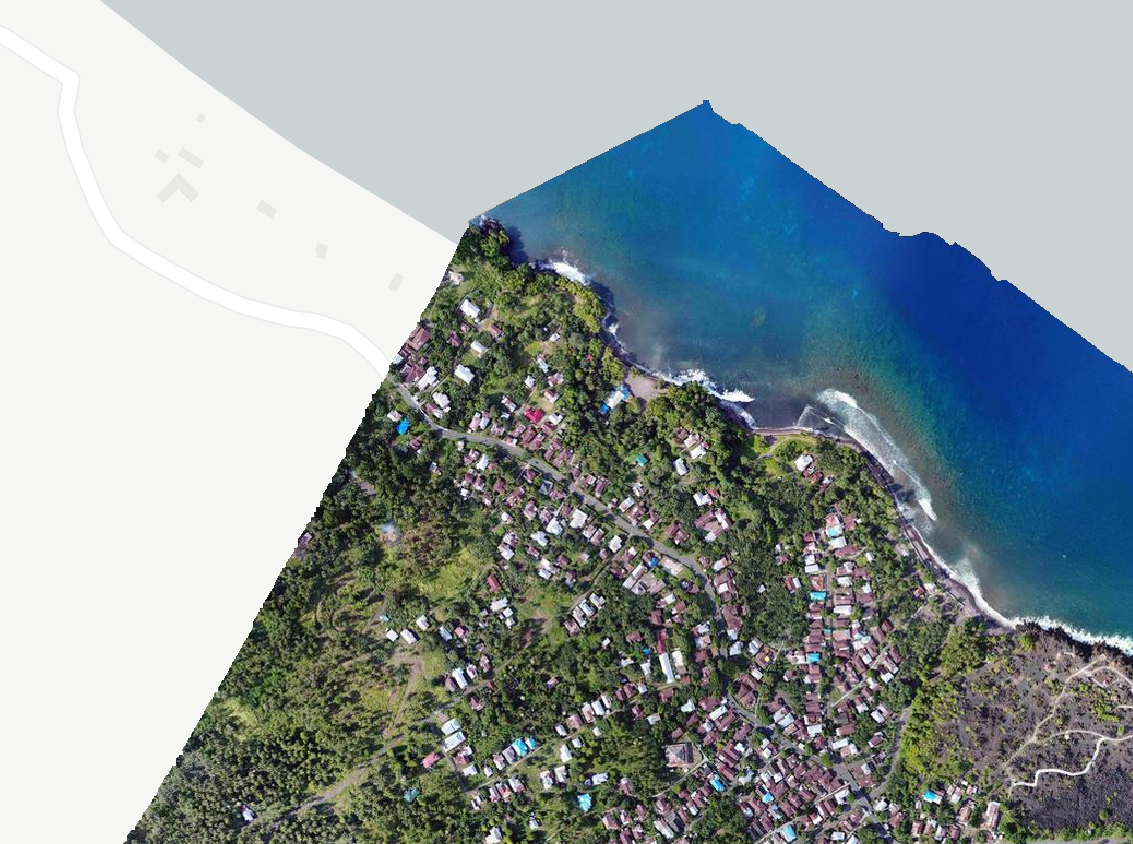
\includegraphics[width=\linewidth]{figs/orthomosaic.png}
  \caption{Orthomosaic. source: Indonesian Redcross/OpenAerialMap}
  \label{fig:orthomosaic}
\end{figure}


\section{Aerophotogrammetry}

Aerophotogrammetry takes the job on step further. By knowing the cameras lens intrinsics, software are capable of matching a number of pictures, detecting features on the environment, and locating the point used to take each of the pictures. With this information, it's possible to rebuild in 3D most of the environments, enabling the operator to interact with the area as a 3D mesh.
By using precise GPS information(such as RTK/PPK data, or total stations) or known landmarks, it's possible to accurately measure distances, areas, volumes, angles and elevations, simplifying the surveyors' job.

Aerophotogrametry can also rebuild in 3D buildings and other structures, 
\chapter{The Requisites} \label{chap:3}


\section{Objective}

%%%%
%%
\section{Requisites}

%%%
%%
\section{Functional Requisites}



%%%%%%%%%%%%%%%%%


\chapter{Flight Mechanics and Design} \label{chap:FlightMechanics}

\section{Brief Introduction to Flight Mechanics}

Flight mechanics deal with a vehicles interaction with propulsional, aerodynamic, and gravitational forces.

In order to achieve proper flight, a vehicle needs an upwards force, and means of maneuverability. the former is usually generated by the means of a propeller, while the latter can be either the result of spinning propellers, or using control surfaces to deflect the passing air movement, causing a force to the opposite direction. 
%
This field of mechanics deals with the study of vehicle trajectories (performance), stability, and aerodynamic
control.


\section{Fixed-Wing Mechanics}

In fixed-wing aircraft, air flowing through the wings generates a pressure differential, usually lowering the pressure on top of the wing, generating a force usually called "lift", the force responsible for canceling the gravitational pull and keeping the vehicle aloft in the air.

In a simplified explanation, two main principles are responsible for generating lift:

\subsection{Flow deflection and Newton's laws}

Most wings have an angle of attack (to be hereafter called $\alpha$ ) such that $\alpha > 0$, which means the air passing through it gets deflected down. According to Newton's second law, an opposite force is necessary on the wing. This force is the generated lift.

\subsection{Increased flow speed and Bernoulli's principle}

Bernoulli's principle states that within a steady airflow of constant energy, when the air flows through a region of lower pressure it speeds up and vice versa. Implying there is a direct mathematical relationship between the pressure and the speed, meaning if one knows the speed at all points within the airflow, on can calculate the pressure and vice versa. For a cambered airfoil (where the chord at the top is longer that the chord at the bottom) the/home/will/Pictures/Screenshot from 2017-11-13 11-03-27.png air needs to take a longer path, moving faster, thus lowering the pressure on the top, and generating lift.


\subsection{Airfoil Shape}
How much lift is generated depends on the chosen airfoil.
%
An cambered airfoil (longer chord on the upper surface than in the lower one) generated lift even when the angle of attack $\alpha$ is zero.
Symmetric airfoils need a positive angle, and the lift is generated by deflecting the air downwards.
Other properties that depend on the airfoil shape are the drag (air force pushing against the direction of movement) and angular moment it generates on the aircraft. 

\subsection{The Coordinate System and Nomenclature}

The coordinate system, when dealing with the fixed-wing mode, is as shown in figure \ref{fig:coords1}

\begin{figure}
\centering
  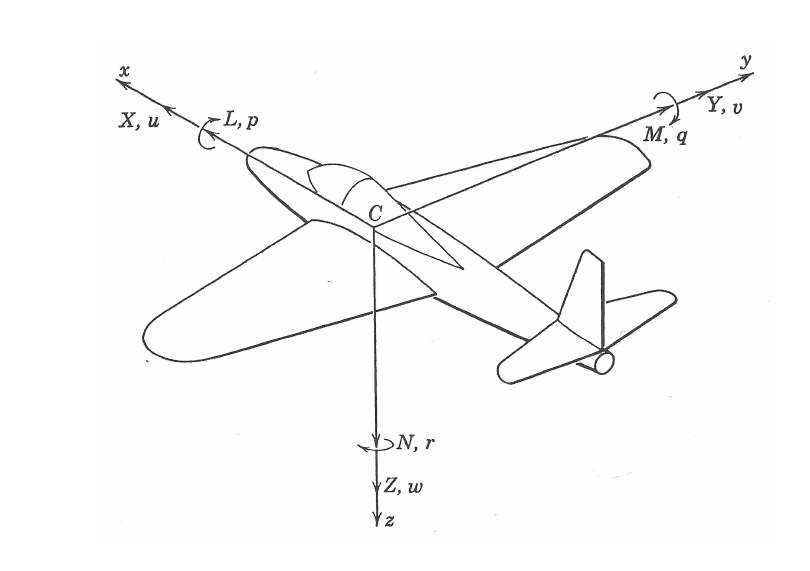
\includegraphics[width=\linewidth]{figs/axis1.png}
  \caption{Coordinates system and relevant variables.}
  \label{fig:coords1}
\end{figure}

Where:


\begin{itemize}

\item $x$, $y$, and $z$ are the coordinates, with the origin in the vehicle's center of mass.
\item $u$, $v$, and $w$ are the linear velocities in each of the $x$, $y$, and $z$ coordinates, respectively.
\item $X$, $Y$, and $Z$ are the components of the aerodynamic force in each of the $x$, $y$, and $z$ coordinates, respectively.
\item $p$, $q$, and $r$ are the linear velocities in each of the $x$, $y$, and $z$ coordinates, respectively.
\item $u$, $v$, and $w$ are the linear velocities in each of the $x$, $y$, and $z$ coordinates, respectively.
\item  Although not indicated in the figure, the variables $\phi$, $\theta$, $\psi$ represent the angular rotations,
relative to the equilibrium state, about the x, y, and z axes, respectively. Thus, $p=\dot{\phi}$, $q = \dot{theta}$
and $r = \dot{\psi}$ where the dots represent time derivatives.

$\phi$, $\theta$, and $\psi$ can also be referred, respectively, as \textit{roll}, \textit{pitch}, and \textit{yaw}.

\end{itemize}

\section{VTOL Mechanics}

When in VTOL mode, the coordinate system used is similar to that in a conventional multirotor, with $Z$ pointing up parallel the motors axis, and $X$ going through the fuselage, pointing away from the belly of the aircraft.

The mechanics involved in vertical take-offs and landings is slightly different. The lift generated becomes meaningless, no more than a slight perturbation to the system. The generated thrust becomes directly responsible for vertical motion and roll control, while the control surfaces can redirect the airflow allowing control of yaw and pitch.

An approximate model can be seen on \cite{7487466}, however, as this work does not focus on the dynamics or control itself, it is not detailed here.


\section{XFLR5}

XFLR5 is an analysis tool for airfoils, wings and planes operating at low Reynolds Numbers. It includes:
\begin{itemize}

\item XFoil's Direct and Inverse analysis capabilities;
\item Wing design and analysis capabilities based on the Lifting Line Theory, on the Vortex Lattice Method, and on a 3D Panel Method.

This tools enables the iterative design and analysis of multiple aircraft configurations.

\todo{elaborar aqui}

\end{itemize}


\section{Design}

The chosen design is the one of a flying wing, a fuselage-less made of a wing, propulsion system, and control surfaces. The reasons are because of a simpler and sturdier mechanical structure, besides the possibility of the VTOL configuration

\subsection{Preliminar Design}

As a starting point, a wing with a central hub and 2 semi-wings ending in symmetrical winglets was designed. The ZAGI12 airfoil was chosen due to it's good soaring capabilities and low stall speed \todo{citation needed}.

With the airfoil chosen, It's characteristics were calculated with the aid of XFOIL, an airfoil analysis tool built into XFLR5.

\begin{figure}
\centering
  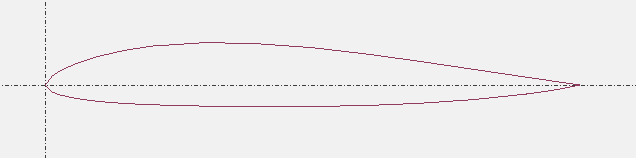
\includegraphics[width=\linewidth]{figs/zagi12.png}
  \caption{Zagi 12 airfoil.}
  \label{fig:zagi12}
\end{figure}


These characteristics plots can be seen on figure \ref{fig:zagi12polares}.
%

It can be noted that the point with the highest Cl/Cd ratio, the theoretical point with better lift to drag ratio, and therefore best gliding performance. It's also notable that the airfoils moment "pulls" it into this better Cl/Cd ratio, allowing the aircraft to fly into this ideal condition without deflection of the control surfaces


\begin{figure}
\centering
  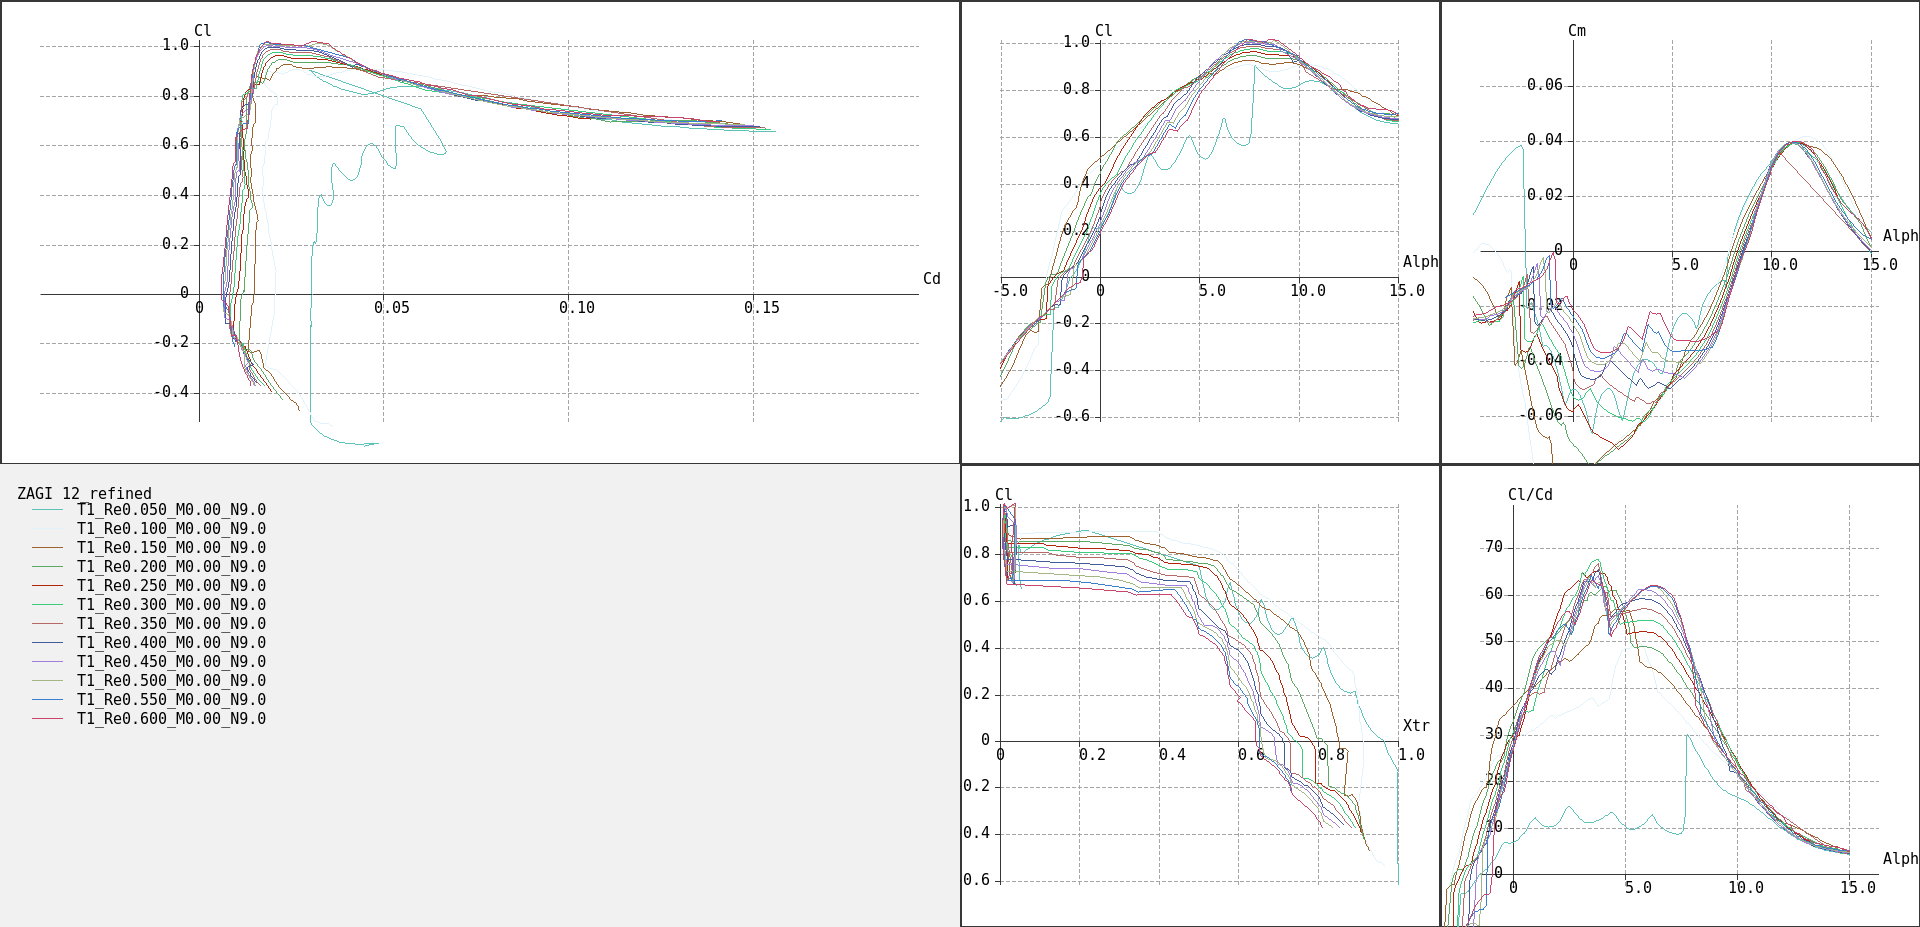
\includegraphics[width=\linewidth]{figs/polares.png}
  \caption{Zagi 12 characteristics}
  \label{fig:zagi12polares}
\end{figure}

With that data, the main body was conceived, as seen in the figure \ref{fig:preliminar}. With this CAD tool we can then analyze the performance of the aircraft as a whole. This gives us the same data as the airfoils', but for the whole craft, as seen in figure \ref{fig:craftpolar}.

Some data can be inferred from these graphs. From \ref{fig:zagi12polares} it can be seen that the highest $C_l$, or Lift Coefficient, is obtained around $\alpha = 8\deg$, which, possibly by design of the airfoil, is also the zone with a higher $C_l/C_d$, or \textit{lift-to-drag ratio} maximizing the gliding distance. It's also notable tat the $C_m  \times \alpha$ plot crosses 0 around the the same $8\deg$, meaning the profile is generally trying to point at that angle.

\begin{figure}
\centering
  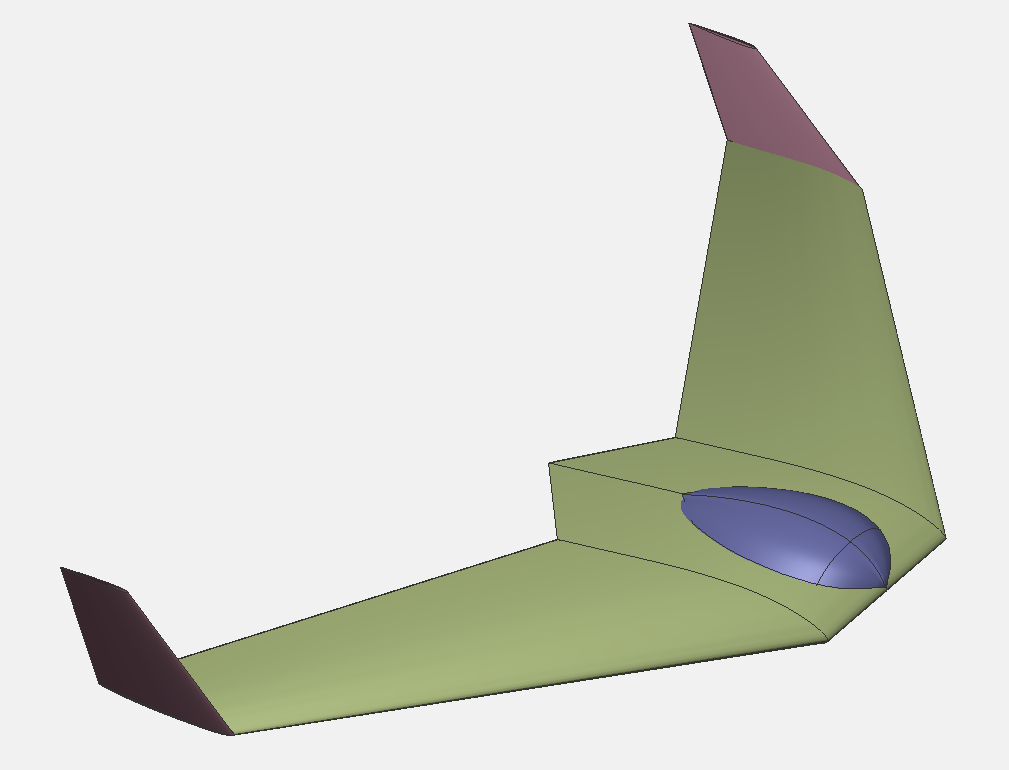
\includegraphics[width=\linewidth]{figs/preliminar.png}
  \caption{First concept of the aircraft.}
  \label{fig:preliminar}
\end{figure}


From \ref{fig:craftpolar}, 	

\begin{figure}
\centering
  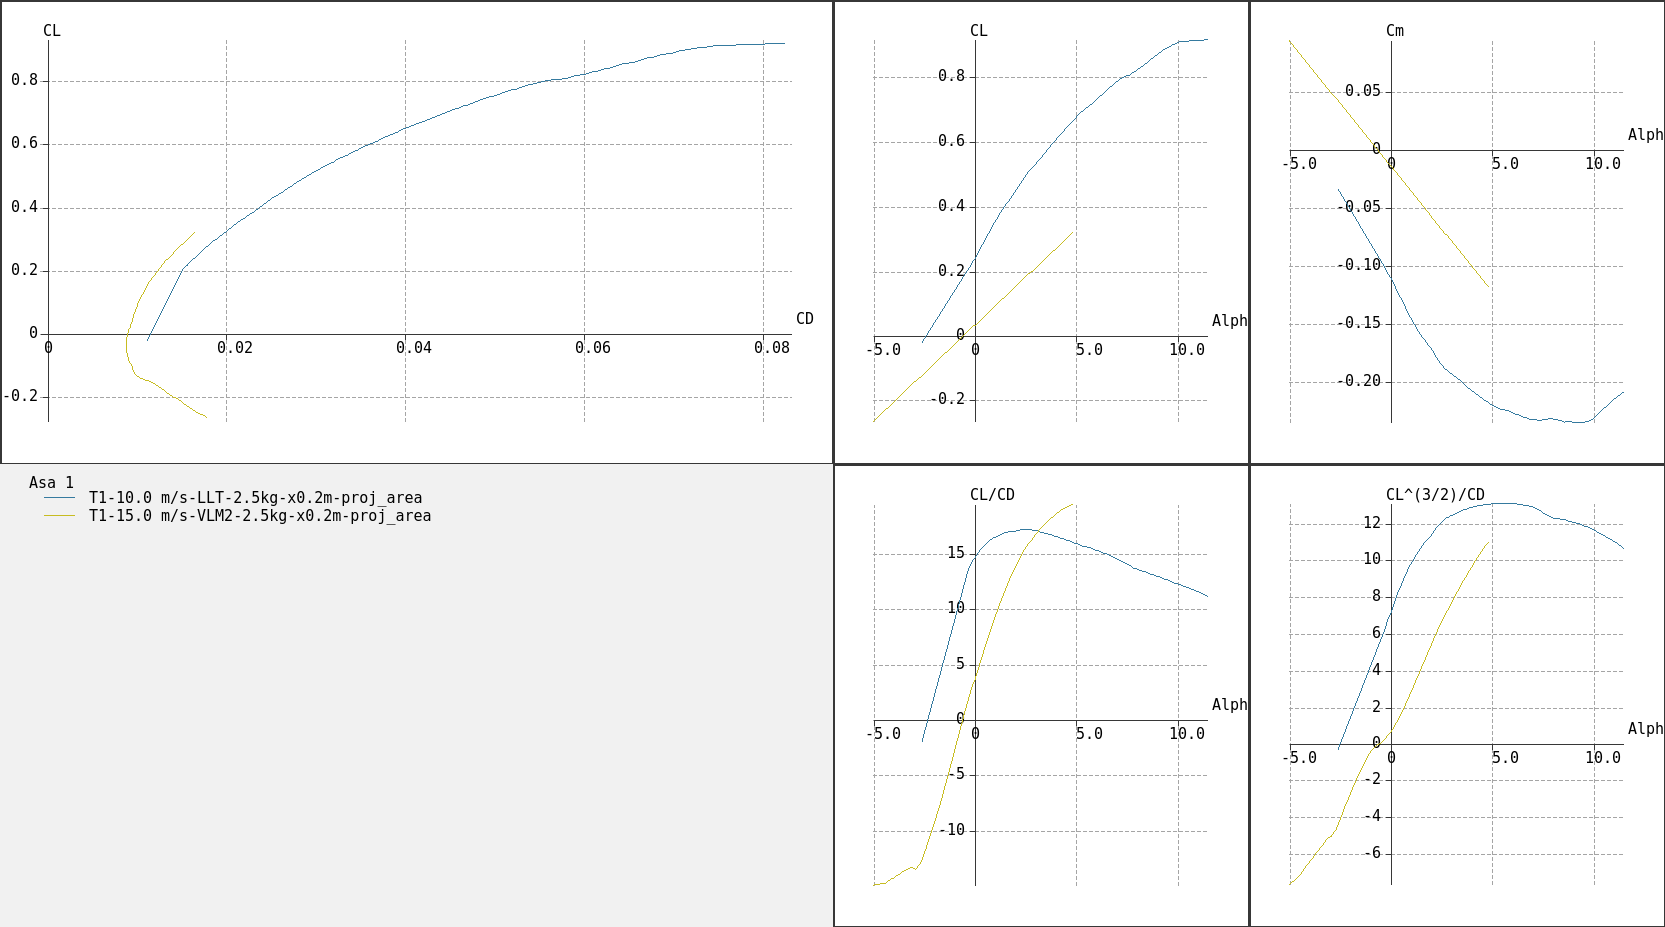
\includegraphics[width=\linewidth]{figs/craftpolar.png}
  \caption{Flight characteristics of the preliminary aircraft design.}
  \label{fig:craftpolar}
\end{figure}


\subsection{Final Design}

Due to building issues and the desire to maximize both effective payload and flight autonomy, the design was simplified, extending the chord back on the beginning of the wings, as seem on figures \ref{fig:final} - \ref{fig:finalrendertop}.
The electronics bay was embedded into the main section, reducing the aerodynamical cross-section, thus reducing drag.
	

\begin{figure}
\centering
  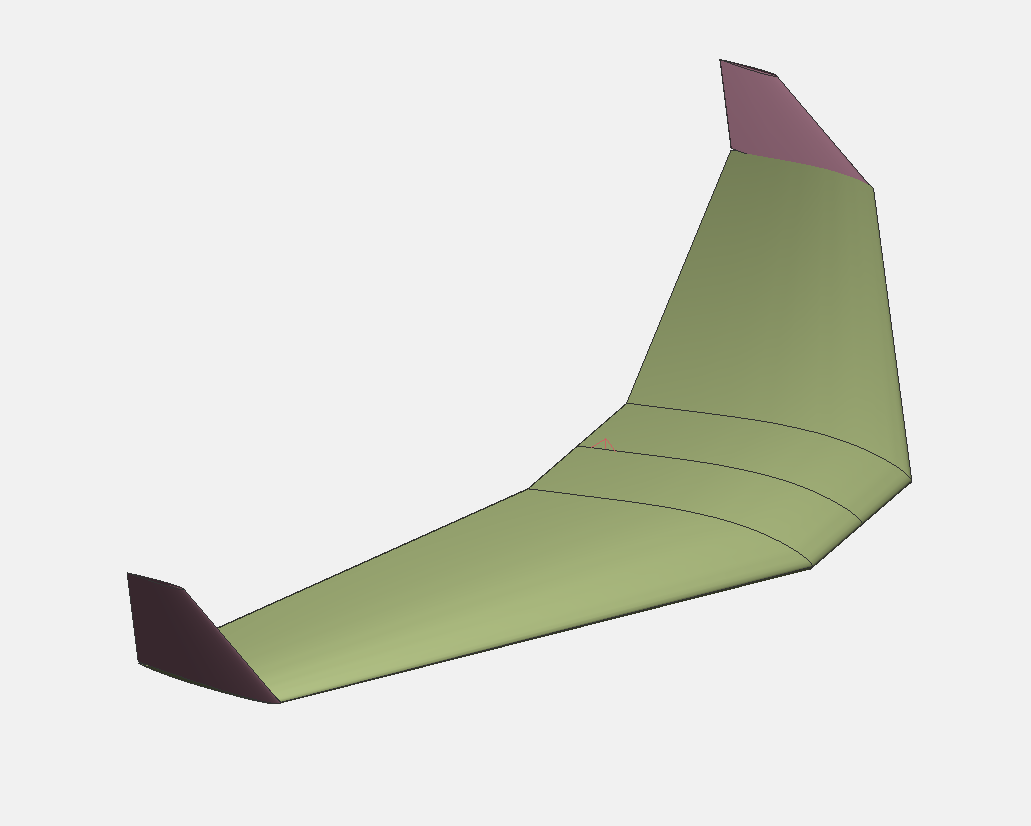
\includegraphics[width=\linewidth]{figs/final.png}
  \caption{Final design of the aircraft, on XFLR5.}
  \label{fig:final}
\end{figure}

\begin{figure}
\centering
  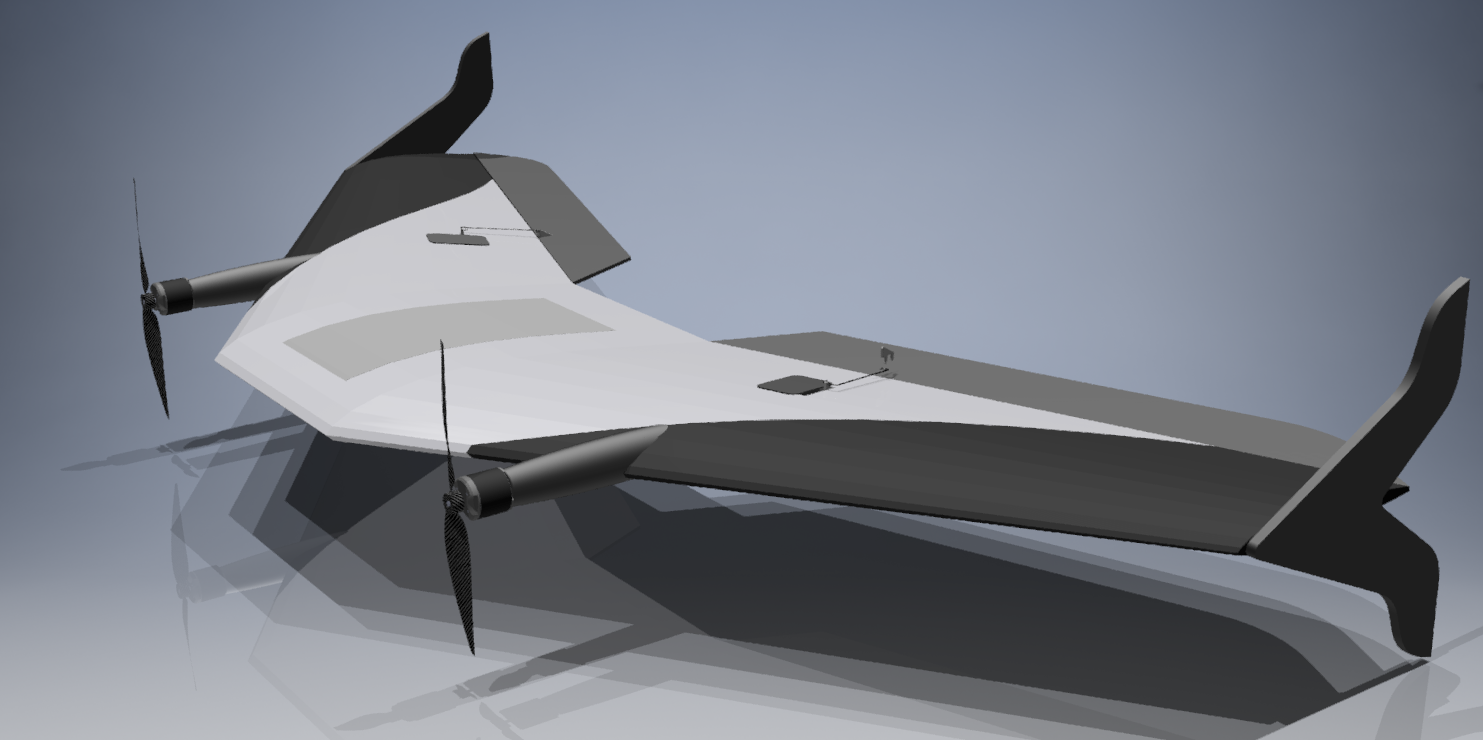
\includegraphics[width=\linewidth]{figs/finalrender.png}
  \caption{Final design of the aircraft.}
  \label{fig:finalrender}
\end{figure}

\begin{figure}
\centering
  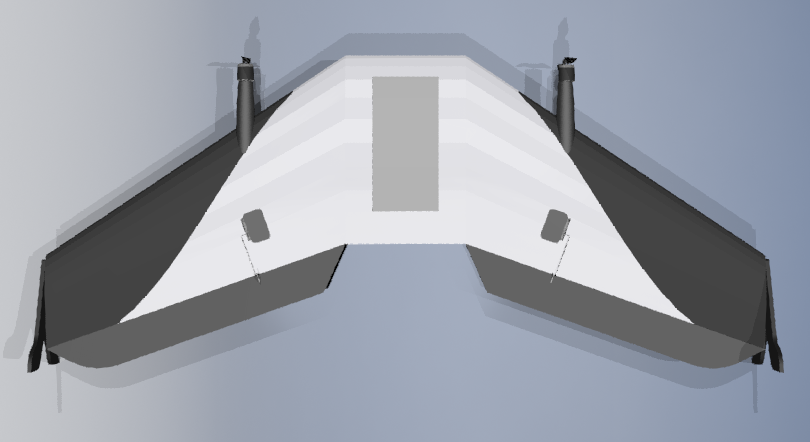
\includegraphics[width=\linewidth]{figs/finalrendertop.png}
  \caption{Final design of the aircraft, top view.}
  \label{fig:finalrendertop}
\end{figure}


%%%%%%%%%%%%%%%

\chapter{The Eletronics} \label{chap:electronics}

In order for the aircraft to fly and navigate autonomously, onboard electronics are required, for both actuation, power source, and navigation. Some of the used electronics were already available, and were chosen for this reason.
	
\section{Propulsion}

Due to the familiriaty and availability, the Mikrokopter Mk3538 Motor was chosen, paired with E-Max Simon 60A escs.

Experimental curves for the motor are available at Mikrokopter's website, and the relevant ones are reproduced on Figure \ref{fig:motorcurves}. Each motor should give, on 25 V, at least 2.2kg of static thrust when paired to 12 inches propellers, up to 3.4 kg on 15 inches, while drawing 34 A, or about 754 W.
\begin{figure}
\centering
  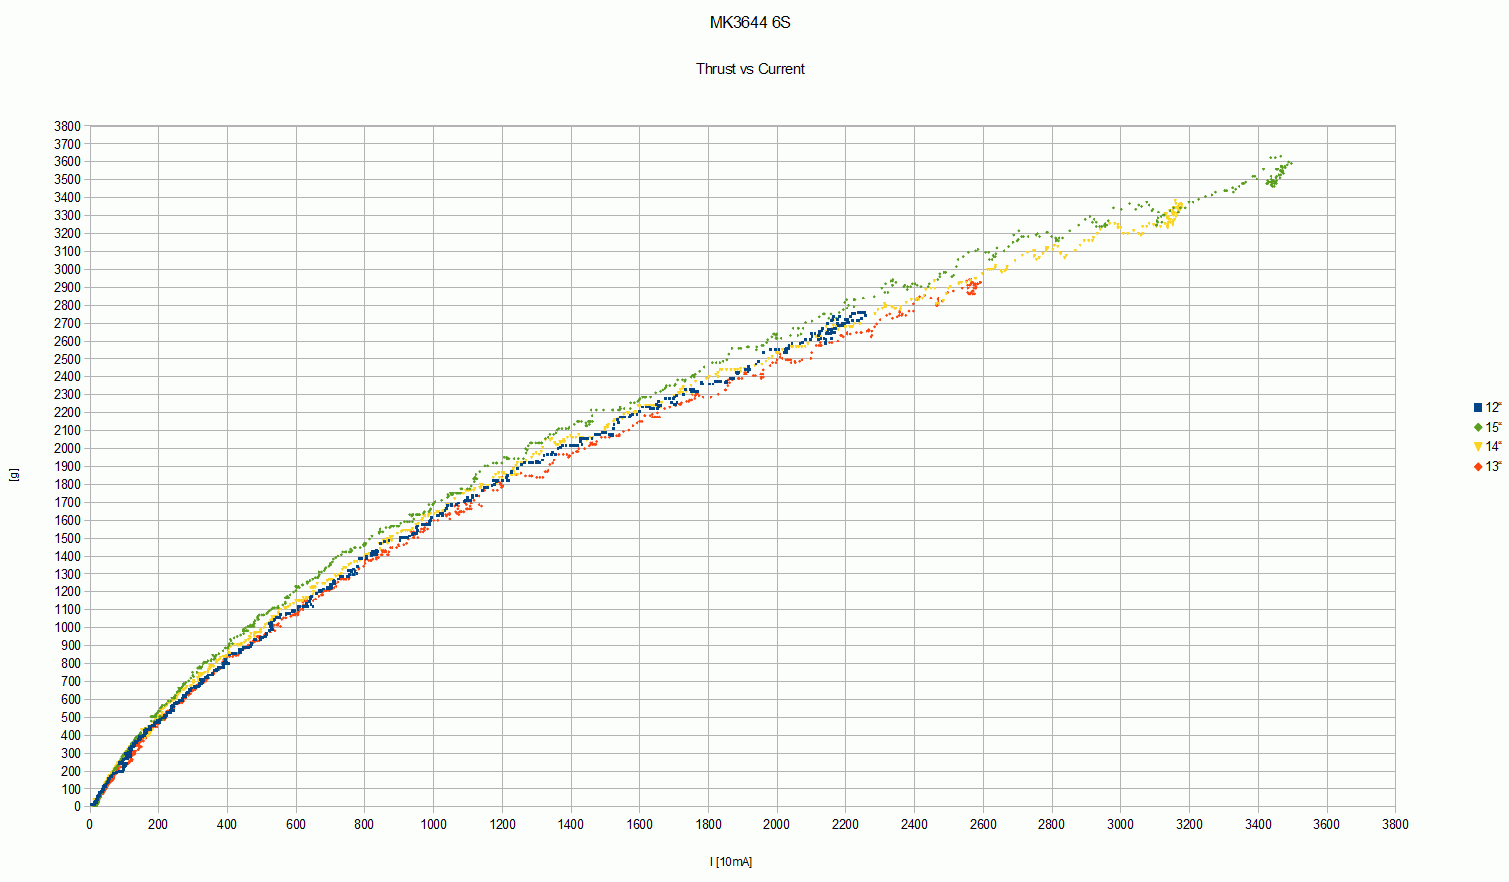
\includegraphics[width=\linewidth]{figs/motorcurves.png}
  \caption{First concept of the aircraft.}
  \label{fig:motorcurves}
\end{figure}


\section{Batteries}

As each motor can draw up to 34 A, the battery should be able to provide up to 68 A without issues.
The Batteries chosen are also the ones already in use by the company, Vislero 4500 mAh 20C, which, at 20 C rating, are able to sustain a constant draw of up to 90 A. 

Each weigh approximately 750 g and measures XXxYYxZZ mm.

\section{The Control Surfaces}

The control surfaces must be slightly larger than usual for a flying wing, as on a tail-sitter a reasonable amount of air must be deflected on hover situation, while on most wings a steady airflow is assumed. It's suggested to have control surfaces taking up to 30\% of the chord of the wings. Since they are easily swappable, it was decided to start with smaller ones, and replace it if necessary

\section{The Flight Controller}

The multirotor had a huge boom last 10 years. In 2009 the first hobby-grade flight controller for multicopters was born, Rolf “KaptainKuk” Bakke's "KK board". Using a simple AVR controller and three gyroscopes, the board could control angular speed on three axis, enabling pilots to control the multirotors. It was programmed in AVR assembly and had individual PID controllers for each axis.
%
Shortly after, Alexinparis noticed the gyros on the Wii Motion + controller, and MultiWii was born. This project grew to support a variety of sensors and boards, and had an active development community, but has now saturated the AVR controller's capability.
%
Shortly after, still in 2010, DIY Drones released the open-source Arducopter, featuring more advanced flight modes, and even autonomous flight.  It did still involve compiling code and flashing it to the controller though.
%
In 2011, DJI started to get visibility with the NAZA controller, which showed remarkable stability, and later got upgraded with a GPS allowing the drone to return to home and hold position in the air. The controller was often sold with a 





The Flight Controller is a PixHawk, running latest Beta release of ArduPlane, where there's experimental support for tail-sitters.


%%%%%%%%%%%%%%%%%%%

% ----------------------------------------------------------
% Finaliza a parte no bookmark do PDF
% para que se inicie o bookmark na raiz
% e adiciona espaço de parte no Sumário
% ----------------------------------------------------------
\phantompart

% ---
% Conclusão
% ---
%\chapter{Conclusão}
% ---

% ----------------------------------------------------------
% ELEMENTOS PÓS-TEXTUAIS
% ----------------------------------------------------------
\postextual
% ----------------------------------------------------------

% ----------------------------------------------------------
% Referências bibliográficas
% ----------------------------------------------------------
\bibliography{bibli}{}

% ----------------------------------------------------------
% Glossário
% ----------------------------------------------------------
%
% Consulte o manual da classe abntex2 para orientações sobre o glossário.
%
%\glossary

\include{apendices}

\include{anexos}
%---------------------------------------------------------------------
% INDICE REMISSIVO
%---------------------------------------------------------------------
\phantompart
\printindex
%---------------------------------------------------------------------

\end{document}
